\section{Security of Global Navigation Satellite Systems --- GNSS}

\paragraph{Overview}
Orbiting satellites transmit their location and a precise timestamp.
Receivers collect these navigation messages and their arrival time and use \textbf{trilateration} to calculate their own position.
\footnote{There are of course issues with special and general relativity that mess with the time.}
Satellites are positioned in such a way that at least four of them are always in sight from any point on Earth. If more satellites are visible, a more precise localization is possible.

Three segments: users, satellites, ground control.

\paragraph{Types of start at the receiver}
\underline{The intuition:} the more the receiver knows, the faster it can lock on to the satellites in view and get a new localization.
\begin{itemize}
	\item \textbf{Cold start:} receiver knows nothing.
	\item \textbf{Warm start:} receiver remembers last calculated position, almanac and UTC time.
	\item \textbf{Hot start:} receiver remembers last calculated position, almanac and UTC time and the last satellites in view.
	\item \textbf{+ Assisted GPS:} receiver gets helped by the cellular network downloading ephemeris and estimating its position using triangulation from cell towers.
\end{itemize}

\paragraph{Signalling}
Each satellite modulates the navigation message with a spreading code (coarse acquisition C/A for civilians (public), precision P/Y for military (secret)). The spread signal is then modulated onto a carrier. Individual satellites use individual spreading codes to allow distinction.

GPS sends on two carrier frequencies at the same time, L1 (1575.42 MHz = 10.23 MHz $\times$ 154) and L2 (1227.60 MHz = 10.23 MHz $\times$ 120).%
\footnote{This only applies to military. The civilian C/A is only transmitted on L1.}
Apart from jamming resistance and redundancy, this also allows to calculate the ionospheric delay error.
\\
Due to atmospheric attenuation, down on Earth the GPS signal is well below the thermal noise.

\paragraph{Navigation message}
Each message consists of 25 frames.
Each takes 30 sec to transmit, so the total time is 12.5 min.
\\
Each frame contains: satellite clock + health data, 2x ephemeris (orbit details), other data + almanac (orbital + clock details).
Navigation messages are transmitted by the satellite at a rate of $50$ bits per second.

\paragraph{Time of Arrival TOA}
The time of arrival is travel time of the signal from the satellite to the receiver and it's used to calculate the distance and, thus, the receiver position. It's found by sliding the spreading code over the received message until a correlation peak is found.

\paragraph{Spoofing attacks}
Messages are unauthenticated (for practical reasons, or else they would become too long).
\\
By sending stronger signals, overshadowing the legitimate ones, an attacker can modify the \textit{navigation message contents} (transmission time, satellite location) or their \textit{time of arrival} (retransmitting captured signals with a temporal shift), resulting in a wrong location being calculated.
\\
This is an issue in civilian GPS (messages can be generated and delayed) as well as in military GPS (messages can only be delayed since they are encrypted).
Unfortunately, commercial GPS signal generators are becoming increasingly cheap.

\paragraph{Impct of attacks}
Jamming can cause DoS, which is bad but it's possible to recover in other ways. However, it's useful to assist other attacks (for example jamming the legitimate signal before injecting a rogue signal).
Obtaining a rogue position is bad for smart/autonomous vehicles, high-value asset tracking especially if you don't detect it and keep trusting the wrong position.
\subsection{Spoofing Detection and Mitigation}\label{sec:gps-spoof}

\paragraph{Types of countermeasures}
\begin{itemize}
	\item \textbf{Infrastructure/protocol:} for example, cryptographic authentication of navigation messages
	\item \textbf{Receivers:} for example, using physical-layer characteristics of the signal to validate the signal as well as the calculated position/velocity/time (e.g.\ direction of arrival, carrier phase, signal strength, etc\dots)
\end{itemize}

\paragraph{Angle of Arrival AoA}
Use multiple antennas (e.g.\ on both ends of a ship) to calculate the angle of arrival through the phase difference and the known distance between the antennas (see beam steering, \autoref{fig:beam-steering}).
In a spoofed scenario, the angles would all be very similar.
Restricts the locations from which the attacker can successfully spoof.

\underline{Problems:}
Attacker can use drones to spoof signal from more realistic angle.
Reflection of legitimate signal of buildings (thus reaching the receiver at a shallower angle) could be wrongly classified as spoofing.
Computationally expensive phase measurement.
Hardware modification.

\paragraph{Monitor Signal Characteristic Changes}
Over time, monitor signal properties such as AGC (Automatic Gain Control), noise level, number of satellites, spatial diversity (AoA) or the autocorrelation peak.
Abrupt changes in any of these indicate presence of spoofing.

\paragraph{Seamless takeover attack}
The attacker starts transmitting a copy of a legitimate GPS signal in sync with the original one, but at low power, having no influence on the receiver.
Then the attacker slowly starts increasing the power, until the receiver prefers the attacker signal.
Now the attacker can change the GPS signal, and the receiver will keep following. 

\begin{figure}[h]
	\centering
	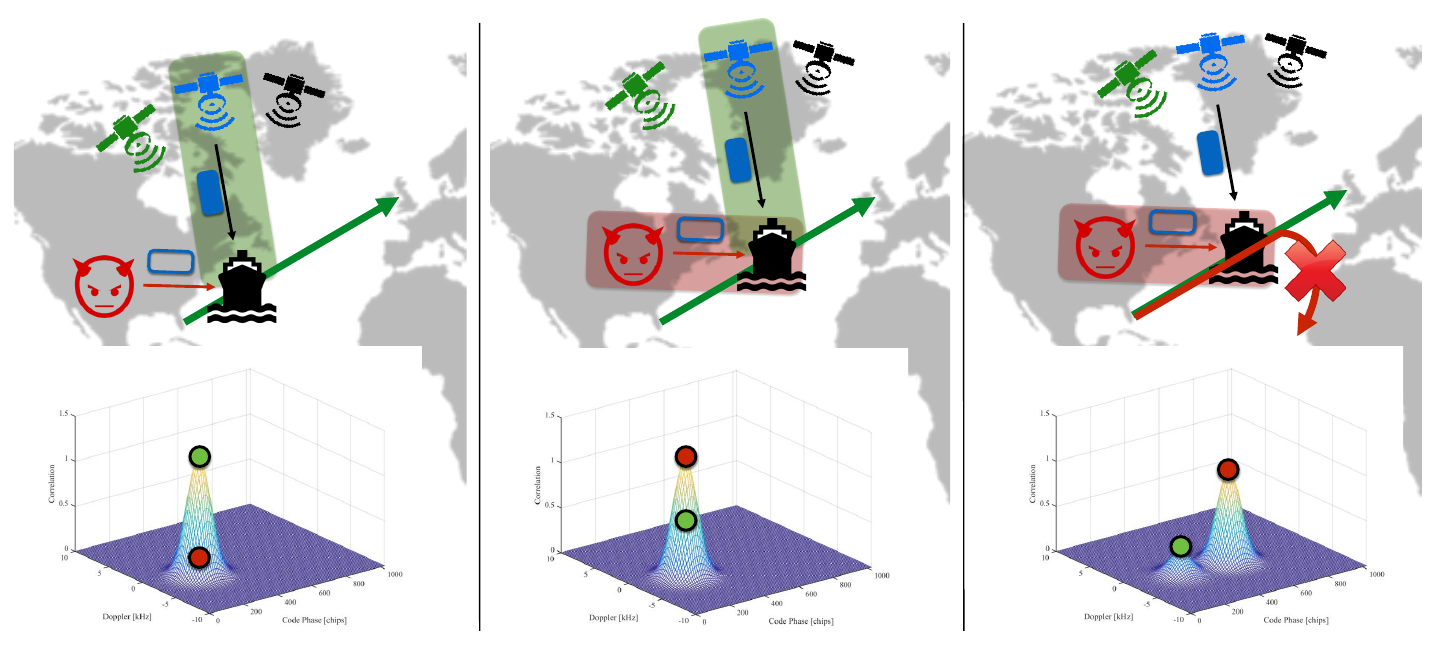
\includegraphics[scale=0.4]{images/4-seamless-takeover.png}
	\caption{Seamless takeover attack}%
	\label{fig:seamless-takeover}
\end{figure}

\paragraph{SPoofing REsistance GPS rEceiver SPREE}
Leverage peak tracking (of \underline{all} signal peaks) to detect seamless takeover attacks.
Navigation message inspection detects content spoofing.

\paragraph{Cryptographic approach (Kuhn)}
\begin{enumerate}
	\item At time $t$: satellite uses secret spreading code.
	Receiver uses a broadband receiver to capture the entire band.
	\item At time $t+dt$: Satellite disclosed code, signing the disclosure with its secret key.
	Receiver verifies signature, de-spreads the signal.
\end{enumerate}

\underline{Advantages:}
Prevents fake signal generation and individual signal delay.

\underline{Disadvantages:}
Requires pre-shared public satellite keys.
Slightly inefficient (longer latency until signal lock).
Requires loose synchronization (after $dt$ the attacker knows the spreading code and can spoof).
Does NOT prevent full-band delay.
Relay/replay attacks (record signal and replay full band in another location in real time).

\paragraph{Galileo OSNMA}
Galileo Open Service Navigation Message authentication offers a way of authenticating messages that's sustainable for the GNSS infrastructure. Solutions that use public key cryptography are not usable since the signatures would be too long to fit in the limited bandwidth available and are computationally too expensive. Symmetric cryptography is not usable as well since it relies on shared secrets that would need to be stored in every receiver, which you can't trust to actually \underline{stay} secret.

OSNMA uses time-delayed authentication. The satellite generates a random value $K_n$ and hashes it $n$ times and obtains a chain. Obviously, the hash function is irreversible, so you can't compute $K_n$ if you have $K_{n-1}$.
The satellite sends the digital signature and then starts sending the messages in the form of \[ M_1, K_0,MAC(M_1, K_1)\] then, after some time, \[ M_2, K_1,MAC(M_2, K_2)\]
Basically, it discloses the key only after the message encrypted with that key has been received --- and thus the key, which is valid only once, is no longer useful to an attacker.
The receiver verifies the first key against the signature using the public key, then verifies the key against the previous key by hashing it and then verifies the previous message using the key disclosed at that moment.

\paragraph{Security analysis}
It's important to note that there are still anticipation attacks which are harder but possible and also delaying attacks, but these can be detected with a clock offset test.
Anticipation attacks (distance shortening) use techniques like Early Detect-Late Commit and Forward error estimation.
